\subsection{Data}
\label{sec:data}

\Cref{tab:data} summarizes the datasets used for training evaluation.


\newcommand{\zoom}[3]{$ #1 \times #2 \times #3 $}
\newcommand{\mr}[2]{\multirow{#1}{*}{#2}}
\newcommand{\mrsp}[4]{\mr{#1}{\zoom{#2}{#3}{#4}}}

\begin{table}
  \footnotesize
  \setlength{\tabcolsep}{6pt}
  \centering
  \caption[Datasets summary]{
    Datasets used in this study.
    Where multiple resolutions are present, the minimum, mean and maximum for each dimension are shown.
    `\acs{T1wCE}' indicates that gadolinium was administered for contrast enhancement.
  }
  \label{tab:data}
  \begin{tabular}{llcrlr}
    \toprule
    \textbf{Dataset} & \textbf{Modality} & \textbf{Resolution (mm)} & \textbf{Subjects} & \textbf{Surgery} & \textbf{Annotated} \\
    \midrule
    \mr{3}{\textbf{IXI}}     &          \mr{3}{\ac{T1w}} & \zoom{0.94}{0.94}{1.20}  &       \mr{3}{566} &          \mr{3}{-} &          \mr{3}{-} \\
                             &                           & \zoom{0.94}{0.94}{1.20}  &                   &                    &                    \\
                             &                           & \zoom{0.98}{0.98}{1.20}  &                   &                    &                    \\
    \midrule
    \textbf{ADNI}            &                  \ac{T1w} & \zoom{1.00}{1.00}{1.00}  &               467 &                  - &                  - \\
    \midrule
    \mr{3}{\textbf{OASIS}}   &          \mr{3}{\ac{T1w}} & \zoom{1.00}{1.00}{1.00}  &       \mr{3}{780} &          \mr{3}{-} &          \mr{3}{-} \\
                             &                           & \zoom{1.05}{1.01}{1.02}  &                   &                    &                    \\
                             &                           & \zoom{1.20}{1.05}{3.00}  &                   &                    &                    \\
    \midrule
    \mr{3}{\textbf{EPISURG}} &          \mr{3}{\ac{T1w}} & \zoom{0.75}{0.75}{0.75}  &       \mr{3}{430} &   \mr{3}{Epilepsy} &        \mr{3}{133} \\
                             &                           & \zoom{0.96}{0.96}{1.08}  &                   &                    &                    \\
                             &                           & \zoom{1.09}{1.09}{1.60}  &                   &                    &                    \\
    \midrule
    \textbf{Milan}           &                  \ac{T1w} & \zoom{0.46}{0.46}{0.90}  &                20 &           Epilepsy &                 20 \\
    \midrule
    \mr{3}{\textbf{Strasbourg}} & \mr{3}{\ac{T1w} \& \acs{T1wCE}} & \zoom{0.23}{0.23}{0.50}  &        \mr{3}{33} &   \mr{3}{Epilepsy} &         \mr{3}{33} \\
                             &                           & \zoom{0.61}{0.61}{2.79}  &                   &                    &                    \\
                             &                           & \zoom{1.00}{1.00}{5.00}  &                   &                    &                    \\
    \midrule
    \mr{3}{\textbf{Paris}}   &          \mr{3}{\ac{T1w}} & \zoom{0.47}{0.47}{0.49}  &        \mr{3}{19} &   \mr{3}{Epilepsy} &         \mr{3}{19} \\
                             &                           & \zoom{0.82}{0.76}{1.06}  &                   &                    &                    \\
                             &                           & \zoom{1.20}{0.98}{1.20}  &                   &                    &                    \\
    \midrule
    \mr{3}{\textbf{BITE}}    &       \mr{3}{\acs{T1wCE}} & \zoom{1.00}{0.47}{0.47}  &        \mr{3}{13} &      \mr{3}{Tumor} &          \mr{3}{0} \\
                             &                           & \zoom{2.31}{0.53}{0.53}  &                   &                    &                    \\
                             &                           & \zoom{5.50}{0.55}{0.55}  &                   &                    &                    \\
    \bottomrule
  \end{tabular}
\end{table}


\subsubsection{Public data for simulation}

\ac{T1w} \acp{MRI} were collected from publicly available datasets \ac{IXI}\fnurl{https://brain-development.org/ixi-dataset/}, \ac{ADNI} \cite{jack_alzheimers_2008}, and \ac{OASIS} \cite{lamontagne_oasis-3_2019}, for a total of 1813 images.

These datasets are used as control subjects in our self-supervised experiments (\cref{sec:sim_res_self}).
Although we use the term `control' to refer to subjects that have not undergone resective surgery, they may have other neurological conditions.
For example, subjects in \ac{ADNI} may suffer from Alzheimer's disease.


\subsubsection{Multicenter epilepsy data}
\label{sec:multicenter}

We evaluate the generalizability of our approach to data from several institutions: \textit{Milan} ($n = 20$), \textit{Paris} ($n = 19$), \textit{Strasbourg} ($n = 33$), and EPISURG ($n = 133$).

We curated the EPISURG dataset using images from patients with refractory focal epilepsy who underwent resective surgery between 1990 and 2018 at the \ac{NHNN}, London, United Kingdom%
\footnote{Informed consent to be included in a research study was obtained from all included patients.}.
These were anonymized data that had been previously acquired as a part of clinical care, so individual patient consent was not required.
All images in EPISURG were defaced using a predefined face mask in the \ac{MNI} space to preserve patient identity (\cref{fig:defacing}).
In total, there were 430 patients with postoperative \ac{T1w} \ac{MRI}, 268 of which had a corresponding preoperative \ac{MRI}.
All the sequences are 1.5-T or 3-T \ac{FSPGR}, \ac{FSPGR} \ac{BRAVO} or \ac{MPRAGE}.
The distribution of resection types is shown in \cref{tab:episurg}.

\begin{figure}
  \centering
  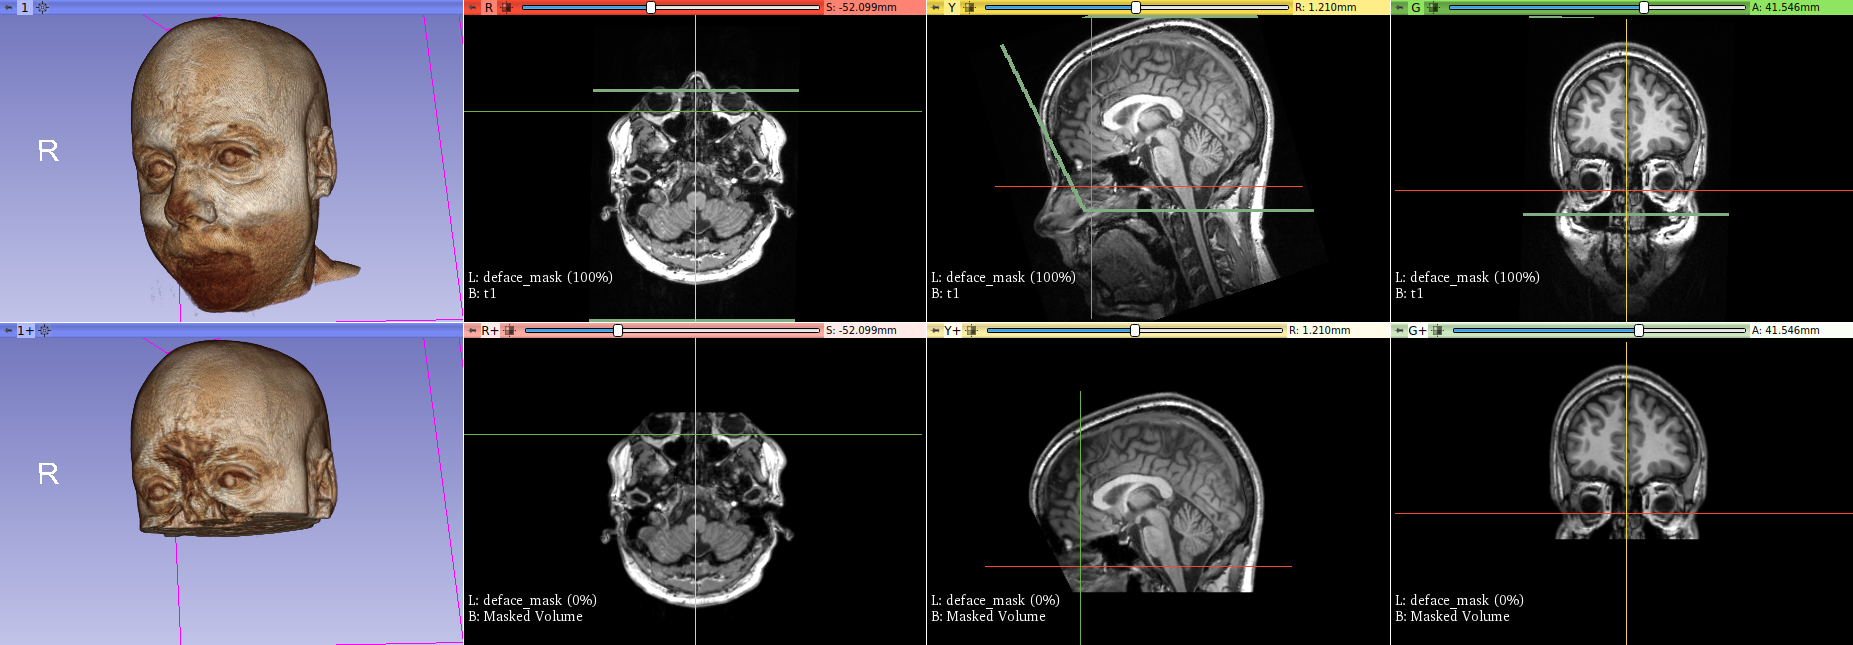
\includegraphics[width=\linewidth]{figures/defacing}
  \caption[Example of a defaced image]{Example of a defaced image. Top: original \ac{T1w} \ac{MRI} with intersection of the defacing mask in green; bottom: result of applying the defacing mask. This use of this image in this report was approved by the subject.}
  \label{fig:defacing}
\end{figure}

% Three human raters performed 200 (133 + 33 + 34) manual annotations of the postoperative images in EPISURG \cite{perez-garcia_simulation_2020}.
Annotations used for evaluation in this study were performed semi-automatically using a fast grow-cut algorithm implemented in 3D Slicer 4.10 \cite{zhu_effective_2014,fedorov_3d_2012}.
The same human rater (F.P.G.) annotated all images from \textit{Milan}, \textit{Paris} and \textit{Strasbourg} using the same protocol that was used for EPISURG.
EPISURG is available online and can be freely downloaded \cite{perez-garcia_episurg_2020}%
\fnurl{https://doi.org/10.5522/04/9996158.v1}.


\begin{table}
  \centering
  \setlength{\tabcolsep}{12pt}
  \caption{
    Lobar distribution of resection types in EPISURG.
  }
  \label{tab:episurg}
  \begin{tabular}{llS[table-format=3.0]}
    \toprule
    \textbf{Lobe}       & \textbf{Type}    & \textbf{Subjects} \\
    \midrule
    Temporal            & Lobe resection   &        317 \\
    Temporal            & Lesionectomy     &         30 \\
    Temporal--frontal   & Lobe resection   &          2 \\
    Temporal--parietal  & Lobe resection   &          1 \\
    Frontal             & Lobe resection   &         47 \\
    Frontal             & Lesionectomy     &         10 \\
    Parietal            & Lesionectomy     &         11 \\
    Parietal            & Lobe resection   &          4 \\
    Occipital--parietal & Lobe resection   &          2 \\
    Occipital           & Lobe resection   &          2 \\
    -                   & Multiple subpial &          2 \\
    -                   & Hemispherectomy  &          2 \\
    \midrule
    \textbf{Total}      &                  &        430 \\
    \bottomrule
  \end{tabular}
\end{table}



\subsubsection{Brain tumor datasets}

The \ac{BITE} dataset \cite{mercier_online_2012} consists of ultrasound and \ac{MRI} of patients with brain tumors.
We use the 13 postoperative \ac{T1wCE} in \ac{BITE} to perform a qualitative assessment of the potential of our models to generalize to images from a substantially different domain (images are contrast-enhanced) and different pathology, which may require different surgical techniques that could affect resection cavity appearance.



\subsubsection{Preprocessing}
\label{sec:preprocessing}

For all images, the brain was segmented using ROBEX \cite{iglesias_robust_2011}%
\footnote{A perfect brain segmentation from resected images is generally not possible due to the missing tissue.
However, the results generated by ROBEX have been useful for a robust registration in our experiments.}.
Voxels within the brain were used to register the images to the nonlinear symmetric ICBM152 \ac{MNI} template \cite{fonov_unbiased_2009,fonov_unbiased_2011} using a pyramidal approach to compute the affine transformation \cite{modat_global_2014}.
All images were resampled into the \ac{MNI} space using sinc interpolation to preserve image quality.
After resampling, images had a 1-mm isotropic resolution and size \zoom{193}{229}{193} voxels.
